\documentclass[11pt,a4paper]{article}
%PKG
\usepackage[utf8]{inputenc}
\usepackage[english]{babel}
\usepackage{amsmath}
\usepackage{amsfonts}
\usepackage{amssymb}
\usepackage{hyperref}
\usepackage{textcomp}
\usepackage{graphicx}

\begin{document}
\graphicspath{{media/}}
\pagestyle{plain}
\author{Axel Jeanne \and Monica Arias Rivera}
\title{Cooperative supervised mobile manipulator}
\maketitle
\begin{abstract}
Robotic systems grew in complexity and diversity due to the increasing complexion of the task
they are performing. As complexity increase, decoupling element into smaller simpler part is
regularly done. As a part if this decoupling trend, cooperative robotics grant an even 
larger change: using multiple robot to perform a single, yet complex, task.

This report present the work performed during the Supervised Mobile Manipulator (SMM) project.
The project consists in making a cooperative robotic system providing "smart" behaviour to
make the tele-operation easier to the user while keeping effectiveness of the controlled robot 
unchanged.

For this project we used different hardware and software elements that we will introduce,
then we will present different cooperative behaviours and will expose their strengths and weaknesses; finally we will present the chosen system and expose its features and the results we obtained.
\end{abstract}
\clearpage

\tableofcontents

\clearpage
\section{Theoretical content}
\subsection{Advantages of cooperative system}
In most cases, the operator performing a task remotely only have a single point of view: the
one of the embedded camera. In multiple different systems, it has been shown that this can
lead to inconvenient situations where the operator is performing a task with a sub-optimal
vision of the situation.

One solution to this problem could be to add an animate vision system\cite{Ballard1991}
but this kind of solution increase vastly complexity of the system since all the vision system
has to be actuated. Another solution could be to increase the number of camera on the robot.
This solution increase the robot payload and is actually not very convenient for the user
since more video streams has now to be monitored while performing the task. The solution we chose is to add an external robot to provide a "supervisor" vision of the acting robot. This solution adds many different  advantages:

\begin{enumerate}
\item The supervisor can provide vision from different angles while the action robot is static
\item The supervisor can scout ahead of the action robot to ensure safety
\item The supervisor behaviours can be automated to unload the operator's attention
\end{enumerate}


\subsection{Problem statement}
The Supervise Mobile Manipulator Project (SMM) goal is to develop a cooperative robotics
system which can be used in hazardous areas. It uses two platforms: 

\begin{itemize}
\item An action platform which perform the physical operation
\item An supervisor platform which keep an overview of the situation
\end{itemize}

To deliver a fully applicable solution, a GUI (Graphical User Interface) had to be provided in
order to see what is the system doing in real time.


\subsection{Tools used}
\subsubsection{Git}
To deliver a complete solution, a lot of software development was required. In order to keep
the code maintained and keep track of changes in code; we used \href{https://git-scm.com/}{git} as a version control system
 (VCS).

\subsubsection{ROS}
\href{http://www.ros.org}{ROS} stands for Robotic Operating System; ROS is not technically a OS but provides many abstraction for network communications among robots. As we require cooperation among our 
system, ROS was a very useful tool.

\subsubsection{Gmapping}
The \href{http://wiki.ros.org/gmapping}{Gmapping} ROS package is an implementation of the Simultanous Localization and Mapping (SLAM) algorithm. It builds a grid map from a laser scan, and localizes the robot from odometry data and features extracted from the environment.

\subsubsection{Navigation Stack}
The \href{http://wiki.ros.org/navigation}{Navigation} ROS package enables a mobile robot to avoid obstacles in the environment based on sensor readings, make a plan to reach a goal and produces appropriate velocities to get there. It accomplishes this through two separate implementations. 

First it builds a global costmap of the perceived environment, and builds a global plan from the current position to the goal based on Djisktra's algorithm, this part is platform independent. 

Secondly it builds a local costmap, taking into account close obstacles and the global plan, and sends the command velocities to the platform. The local planner is  platform dependant, and has to be tuned for optimal performance.

\subsubsection{Tum Ardrone}
The \href{http://wiki.ros.org/tum_ardrone}{Tum Ardrone} ROS package provides a PID controller for the AR Drone, coupled with a state estimation implementation with Extended Kalman Filter (EKF) and Parallel Tracking and Mapping (PTAM).

\subsubsection{Gazebo}
Gazebo is a well known and widely used simulator with a robust physics engine. 
Robot platforms like the TurtleBot and the AR Drone are already implemented, and new robots can be added using a SDF description. It also counts with different plugins  for robot, sensor, and environmental control. 

\subsubsection{Qt}
Qt is a well known GUI library. Is is used a large variety of applications from mobile phone interfaces to advanced customized programs. Qt is so popular that a module for ROS was
created called rqt (ROS Qt).


\subsection{Mobile base}
\begin{center}
Image here
%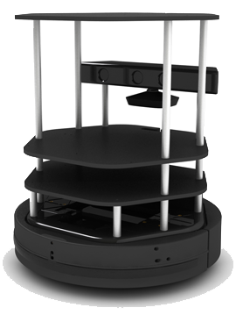
\includegraphics{turtlebot.png}
\end{center}
The mobile base used is a TurtleBot. TurtleBot is a low-cost, personal robot kit with open-source software
provided by different partners mostly for educational activities.
Our mobile base was equipped with a Microsoft\textcopyright Kinect\texttrademark : a cheap camera which is
able to compute the depth of an image easily. Having such information is very interesting for navigation
purpose since the relative distance to object is easily accessible.

\subsection{Quadrotor}
\begin{center}
Image here
%\includegraphics{ar_drone_gps_edition.png}
\end{center}
The quad-rotor used is a Parrot\textcopyright AR Drone v2\texttrademark it is a 4 propellers
drone which has a ROS compatible driver. It is also equipped with two cameras: one in front
and another in the bottom. The bottom camera can be used for visual tracking and the drone
has an on-board tracking system, allowing a decent tracking without latency issues.

Additionally, some ROS libraries have been created to be compatible with the drone; we used
one of them called \href{"http://wiki.ros.org/tum_ardrone"}{"tum\_ardrone"} in parallel with
the driver package: \href{"https://github.com/AutonomyLab/ardrone_autonomy"}
{"ardrone\_autonomy"}.

\subsection{Cooperative behaviour}
As the two robots have to cooperate to perform their common goal, it was required to implement
cooperative behaviors on the system. During the conceptualization of the project we established different
cooperative behaviors that the system should be able to manage:

%\begin{itemize}
%\item Default mode
%\item Coupled mode
%\item Decoupled mode
%\item Assistance mode
%\end{itemize}

\subsubsection{Default mode}
The default mode is the one in which the system start. No particular behavior is expected but the two
robots should establish connection and start exchanging their respective localization and status data.

\subsubsection{Coupled mode}
In this mode, the navigation of the two robots is linked, the mobile-base robot has asked the drone to 
rally on top of its position and the drone is tracking the mobile base underneath. From this point if the mobile base moves, the drone remains on top of it and move along.

\subsubsection{Decoupled mode}
This mode is the same as default mode in terms of behaviour. The only difference is that the default mode
is not accessed anymore after start-up. The system will enter the decoupled mode. The two robots movements
are decoupled and can be separately controlled, either by tele-operation or any other method.

\subsubsection{Assistance mode}
The assistance mode is a semi-operated mode. In this mode, the drone will adopt a set of pre-defined
positions around the mobile base. For instance in the case of navigation, the drone will move among a semi-circle (or full circle) behind (around) the mobile platform, allowing the operator to have a better awareness of the situation.
\begin{center}
Image here
%\includegraphics{assistanceBahavior.png}
\end{center}
Additional behaviors can be added into the assistance mode to be even more effective, for instance
adopting a lateral camera position while the robot is grasping an object. This would allows the operator
to have a real-time visual feedback on its action. Another behavior could be "forward scouting" allowing the drone to explore the area before engaging the mobile base.


\section{Work achieved}

\subsection{GUI programming}
Programming the GUI was facilitated by the rqt package. Setting up the interface was, however, a complicated task since the tutorial of rqt is not exactly finished and omitted crucial setup details.

Once the first test widget were operational, the development of the could start.
\subsection{Robots interactions}
\subsection{Simulator implementation}
\subsection{Testing and first results}

\section{Result analysis and conclusions}
\subsection{Final results analysis}
\subsection{Improvement and future work}
\subsection{Conclusion}


\bibliography{bib}
\bibliographystyle{abbrv}
\end{document}
